\chapter[Referencial Teórico]{Referencial Teórico}

\section{Considerações Iniciais}

Neste capítulo, são apresentadas as bases teóricas para a elaboração do 
aplicativo com o objetivo de facilitar o entedimento dos termos utilizados. 
O capítulo está estruturado em seções. Na seção 2.2, serão apresentados os 
conceitos sobre o ciclo menstrual feminino e suas fases e na seção 2.3, serão 
apresentados os fundamentos sobre o Sistema de Recomendação e alguns algoritmos 
utilizados nessa área.

\section{O Ciclo Mentrual}

O ciclo menstrual é um fenômeno biológico que ocorre em mulheres saudáveis
na qual a característica notável é o fluxo sanguíneo vaginal \cite{guyton2012}.
Ele é cíclico e ocorre como resultado direto de variações das concentrações
hormonais secretadas pelo eixo hipotálamo-hipófise-gonadal. Estudos sugerem
que essas flutuações hormonais, principalmente de estrogênio e progesterona,
que ocorrem no decorrer do ciclo, podem influenciar as emoções,
comportamento e a cognição das mulheres \cite{poroma2014}, afetando
diretamente o seu dia-a-dia, como por exemplo, o desempenho nas tarefas
cotidianas ou relacionamentos interpessoais.


O ciclo ideal tem como base 28 dias. Por convenção o primeiro dia de
menstruação é a marca do início do ciclo e a marca do final do ciclo
anterior, caso não tenha ocorrido a gravidez \cite{lenton1984a}. O ciclo
pode ser dividido em duas fases, a fase folicular e a fase lútea
\cite{brondin2008}. O período da menstruação está presente no início da
fase folicular e o período da ovulação está situado entre as duas fases.
Mais informações sobre as fases, quanto tempo elas duram, quais hormônios
atuam, e a influência deles nas mulheres, serão pontuadas nas subseções
seguintes.


\subsection{Fase Folicular}

A fase folicular é a primeira fase do ciclo menstrual, começa com o início
da menstruação e termina com a ovulação. Enquanto ocorre a menstruação e os
hormônios estimulantes dos ovários(principalmente FSH) estão em concentração
baixa, a fase é referida como fase folicular inicial \cite{lenton1984a}.

Essa é a fase responsável pelo desenvolvimento de folículos, dos quais um
será selecionado e se transformará em um óvulo(corpos lutem), que dará início
a ovulação. Os folículos se desenvolvem em resposta ao aumento do hormônio
folículo-estimulante (FSH) (vide Figura \ref{fig01}). Assim que um desses folículos for selecionado, o FSH diminui gradativamente, e progressivamente a produção de
estrogénios começará a aumentar. Os estrogénios produzidos pelo folículo em
crescimento são responsáveis também pelo desenvolvimento do endométrio. Essa fase é normalmente referida como fase folicular tardia.


Normalmente, mulheres de 18 a 24 anos com ciclo de 28 dias tem a fase com
o comprimento de 14 dias, e mulheres de 40 a 44 anos tem de 10 dias
\cite{lenton1984a}, o que indica a diminuição progressiva do tamanho da
fase folicular com o avanço da idade. Em mulheres jovens, a diferença no
tamanho do ciclo é normalmente provocada por ciclos mais curtos ou mais
longos na fase folicular \cite{lenton1984a}. Ciclos irregulares também
costumam ser pela variação no tamanho da fase folicular, enquanto a fase
lútea segue normalmente com tamanho fixo de 14 dias.


\begin{figure}[h]
	\centering
	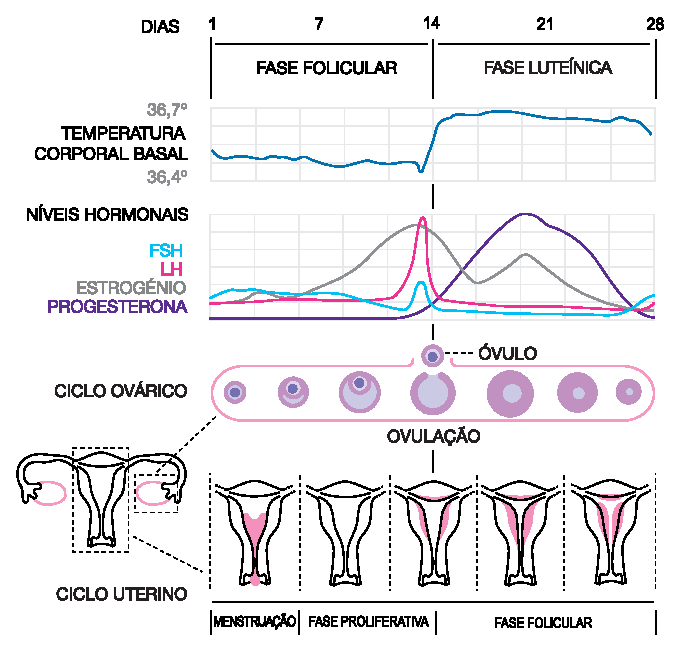
\includegraphics[keepaspectratio=true,scale=0.8]{figuras/MenstrualCycle2_pt.eps}
	\caption{Ciclo Menstrual}
        \label{fig01}
\end{figure}

Alguns estudos demonstraram que no domínio cognitivo 
as funções verbais, espaciais e de memória variam ao longo do ciclo 
menstrual. Na fase folícular, ou quando há baixos níveis de estradiol, 
uma melhora no desempenho em tarefas espaciais foi relatada 
\cite{hausmann2000,maki2002, courvoisier2013, becker1982, phillips1992}, 
e uma melhora nas habilidades verbais foi identificada 
no final da fase folicular quando há altos níveis de estradiol 
\cite{Rosenberg2002}. No aspecto emocional, alguns estudos relacionaram a 
fase com um aumento na habilidade de reconhecimento facial de emoções 
\cite{derntl2013}. Por fim, dois trabalhos concluem que a realização das tarefas verbais é melhor 
ao final das fases folicular e lútea \cite{Rosenberg2002, solis2004}.


\subsubsection{Menstruação}

A menstruação marca o início do ciclo menstrual e o fim do ciclo anterior 
e é caracterizada pelo fluxo sanguíneo vaginal. Ocorre quando não há 
fecundação no ciclo anterior e é composta por sangue e tecido uterino 
derivado da descamação das paredes internas do útero(endométrio). 
Normalmente, dura cerca de 5 dias, mas pode variar \cite{guyton2012}.

O fluxo do sangramento também varia muito, mas costuma ser mais intenso nos primeiros dias. O fluxo menstrual pode ser leve, moderado ou intenso.

\subsection{Ovulação}

A ovulação em si não é uma fase, propriamente dita, mas quando referida 
como tal carrega o significado de um período estimado em que há a 
possível liberação do óvulo e maior probabilidade de gravidez. 
A fase também é referida como fase fértil e, neste estudo, é dividida em 
outra fase por sua importância.

A ovulação acontece pelo equilíbrio entre vários hormonios. 
Clinicamente é possível determinar o ciclo ovulatório pelo surgimento do 
LH e a secreção de progesterona da fase lútea \cite{fritz2010}. 
Quando o estradiol chega ao pico, passadas 12 a 14 horas, o LH surge. 
Na sequência, de 10 a 12 horas depois, faz com que o ovócito complete a 
sua maturação, rompendo o folículo. O folículo é liberado na cavidade 
abdominal, dirigindo-se à trompa de Falópio \cite{fritz2010}. 
A subida do LH é o que determina o início da fase lútea.

Como através de um aplicativo não é possível medir o aparecimento do LH 
para determinar o fim da fase folicular e o início da ovulação, 
e a ovulação é estimada através de uma janela, então a ovulação e a fase 
folicular acabarão se sobrepondo nesse estudo.

\subsection{Fase Lútea}

Com o evento da ovulação, o folículo transforma-se em um corpo lúteo, e as 
células das paredes do folículo começam a produção de progesterona para 
preparar o endométrio para a chegada do óvulo no caso de concepção. 
O pico da progesterona se dá normalmente por volta do vigésimo primeiro 
dia do ciclo \cite{nikas2003}. Caso não haja fecundação, a progesterona 
decai progressivamente e causa novamente a menstruação, continuando assim 
o ciclo.

A fase lútea tem duração de 14 dias e costuma ser constante nas mulheres, 
sem grande variação, mesmo que o tamanho do ciclo varie. É comum no final 
da fase lútea o aparecimeno do transtorno disfórico pré-menstrual(TPM), 
que também ifluência significativamente os aspectos emocionais e 
comportamentais durante as fases do ciclo menstrual. Esse transtorno 
será mais detalhado na sessão 2.2.3.1.

Alguns estudos demonstraram que no domínio cognitivo, as funções verbais, 
espaciais e de memória variam ao longo do ciclo menstrual. Na fase Lútea, 
uma melhora no desempenho em tarefas verbais e memoriais foi relatada 
\cite{hausmann2000}. No aspecto emocional, existe uma piora na precisão 
do reconhecimento de emoções faciais, principalmente para emoções negativas, 
e existe um aumento na memória emocional, principalmente a recordação de 
itens negativos ou detalhes periféricos. As mulheres tendem a responder 
mais rapidamente a situações tristes e estressantes ou expressões faciais 
tristes. Relatou-se que quando os níveis de progesterona estão altos, as 
mulheres demonstram uma maior tendência a perceber expressões de medo. 
Também há evidências que o cortisol, hormônio do estresse, parece se elevar 
na fase lútea\cite{kirschbaum1999}.

\subsubsection{Tensão pré menstrual e o Transtorno Disfórico Pré Menstrual}

Cerca de 90\% das mulheres em idade reprodutiva experienciam algum tipo de 
sintoma pré-menstrual. Uma menor parcela atende aos critérios da tensão 
pré-menstrual(TPM), e cerca de 10\% são diagnosticadas com o transtorno 
disfórico pré menstrual \cite{mishell2005}. Os sintomas pré-menstruais 
são caracterizados com uma lista de sintomas físicos, cognitivos, 
afetivos e comportamentais que ocorrem ciclicamente e aparecem durante a 
fase lútea \cite{obrien2011}, de uma a duas semanas antes da menstruação. 

Os sintomas da TPM variam entre: depressão, irritabilidade, ansiedade, 
explosões de raiva, retraimento social, sensibilidade mamária, 
inchaço abdominal, dores de cabeça e entre outros. Mais de 200 sintomas 
são ligados a essa síndrome. De acordo com o boletim da ACOG, a TPM pode 
ser diagnosticada se um ou mais desses sintomas forem reportados cinco dias 
antes do início da menstruação, durante três ciclos menstruais. Os sintomas 
devem ser registrados por pelo menos dois ciclos; devem passar dentro de 
4 dias após o início da menstruação, e retornar apenas depois do 12º dia do 
ciclo \cite{ACOG2000}.

Não existe um teste laboratórial específico que pode ser utilizado para 
diagnóstico da síndrome, mas a organização mundial da saúde utiliza o ICD-9 
código 635.4 para caracterizar a TPM e o Transtorno Disfórico Pré Menstrual(TDPM). Não existe separação no diagnóstico entre a TPM e a TDPM \cite{biggs2011}.

\subsection{Método Baseado em Calendário}

Apesar de na literatura sobre fertilidade o método preferido para capturar 
a fase do ciclo menstrual ser o uso de medidas diárias dos níveis 
de hormônios combinados ao ultrassom vaginal, para acompanhar o 
desenvolvimento folicular \cite{ecochard2001}; ou ainda a
combinação de medidas hormonais, temperatura corporal Basal e o método 
baseado em calendário \cite{becker2005}, o aplicativo tem a limitação de 
não poder realizar medidas hormonais, nem ultrassons. Adicionalmente, 
o aplicativo não pode contar sempre com a Temperatura Basal Corporal (TBC) 
da sua usuária. Portanto, o método escolhido para classificar as 
fases do ciclo foi o método baseado em calendário.


Nesse método, uma contagem através do calendário é usada para determinar 
a fase do ciclo. O auto-relato do primeiro dia de menstruação é 
utilizado como ponto inicial do calendário, e as fases são determinadas 
contando-se \lq \lq n\rq \rq  números de dias para frente ou de trás para 
a frente a partir da data de início prevista para o próximo ciclo \cite{wideman2013}.


O ciclo base utilizado é normalmente o de 28 dias. Para representar eventos
ovulatórios (próximos a altos níveis de estradiol, e antes de um aumento significativo da
progesterona), é contado 10 a 14 dias a partir do início do ciclo ou de 12 a 14 dias a partir do
dia de previsão para o início do próximo ciclo. Entretanto, enquanto os eventos ovulatórios ocorrem
em média entre esses dias, o momento real da ovulação pode variar significativamente
a partir desta janela. O meio da fase lútea, em que os hormônios ficam 
estabilizados, normalmente é contado de 17 a 21 dias do início do ciclo 
ou de 7 a 9 dias a partir do final do ciclo \cite{wideman2013}. 
A Figura \ref{fig02} representa um ciclo de 28 dias.

Como normalmente a diferença de tamanho dos ciclos dá-se por um aumento 
no tamanho da fase folicular \cite{lenton1984a}, para ciclos maiores ou 
menores que 28 dias a ovulação é adiantada ou atrasada pela diferença 
entre o tamanho do ciclo e o ciclo base de 28 dias. Por exemplo, se for 
um ciclo de 32 dias, a ovulação provavelmente ocorrerá entre o 10º e 18º dia 
a partir do início do ciclo.

\begin{figure}[h]
	\centering
	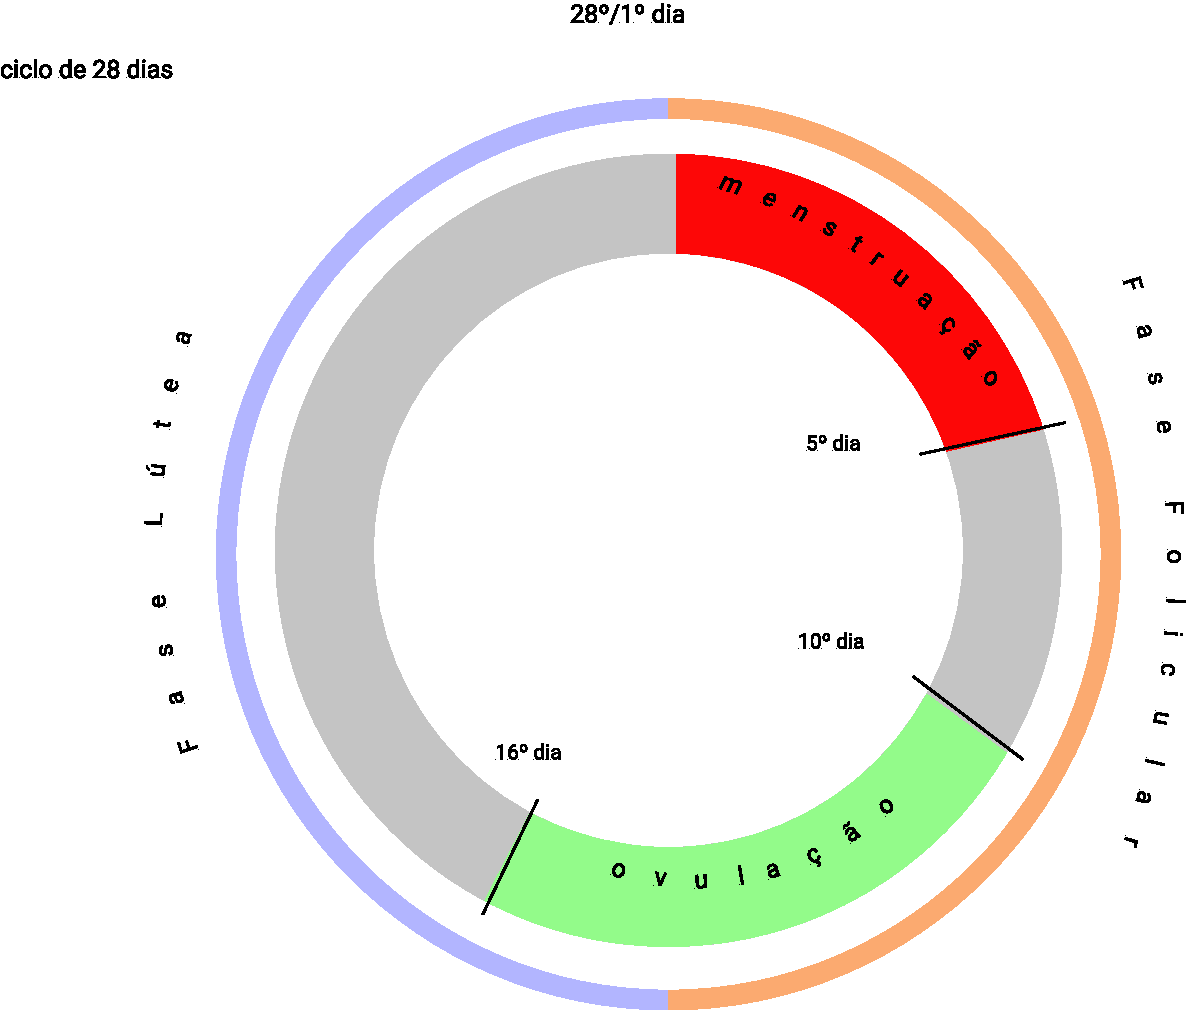
\includegraphics[keepaspectratio=true,scale=0.4]{figuras/Group1.pdf}
	\caption{Calendário do Ciclo Menstrual e Suas Fases (Fonte: Elaborado pela Autora.)}
        \label{fig02}
\end{figure}

\subsection{Outros Fatores que Influenciam no Ciclo Menstrual}

Existem alguns outros fatores que provocam mudanças no ciclo menstrual 
natural da mulher. Nessa seção, são destacados os métodos 
contraceptivos hormonais e distúrbios hormonais.

\subsubsection{Métodos Contraceptivos}

\subsubsection{Disturbios hormonais}

\section{Sistema de Recomendação}
 
Os sistemas de recomendação(SR) tiveram início em meados dos anos 90 
quando os primeiros trabalhos sobre filtragem colaborativa(FC) 
apareceram \cite{felferning2008} evoluídos pelas academias, 
que continuaram desenvolvendo novas abordagens. 
Ainda é uma área de grande interesse devido à grande quantidade de 
problemas que a envolve e por sua praticidade em lidar com o grande 
número de informações disponível na internet \cite{adomavicius2005}. 
O sistema de recomendação veio ajudar os usuários a lidarem com esse 
excesso, fornecendo recomendações personalizadas baseadas nas informações 
coletadas, equilibrando fatores como precisão, novidade, dispersão e 
estabilidade\cite{bobadilla2013}.

Os sistemas de recomendação são implementados e possuem literatura 
para áreas de diferentes temas, como música, televisão, livros, 
documentos, \emph{e-learning}, \emph{e-comerce}, aplicações em mercados, 
pesquisa na web e filmes. A maioria dos estudos estão focados 
para recomendação de filmes \cite{bobadilla2013}.
 
Os sistemas de recomendação coletam informações sobre as preferências 
de seus usuários para um conjunto de itens (livros, filmes, músicas, 
memes, aplicativos, entre outros), e usam de recursos demográficos dos 
usuários (idade, nacionalidade e sexo), informações sociais 
(seguidores, postagens, seguidos), ou informações coletadas através da 
internet das coisas(localização, gps, rfid, sinais de saúde em tempo 
real e outras coisa). Essas informações podem ser adquiridas de maneira 
explicita, por meio de classificações dos usuários, ou implicitamente 
\cite{bobadilla2013}.


De acordo com \citeonline{bobadilla2013}, os sistemas de recomendação 
acompanham a evolução da web. A evolução da web é constituída de três 
fases, a web tradicional, a web social e a internet das coisas. 
Na primeira fase, a geração de sistemas de recomendação usava de 
sites tradicionais para coletar informações de três fonte: dados 
baseados em conteúdo de produtos comprados ou usados; dados 
demográficos coletados nos registros dos usuários, e dados baseados em 
memória, sendo coletados das preferências de itens dos usuários. A segunda 
geração veio com a web 2.0 reunindo informações sociais. A terceira 
geração usa a web 3.0 através de informações fornecidas pelos dispositivos 
integrados na internet(internet das coisas).


Os primeiros sistemas de recomendação focavam em melhorar a precisão da 
recomendação através da filtragem. A maioria dos metodos e algorítimos 
baseados em memória (ex. o KNN, método de agregação, decomposição do valor 
singular, métodos baseados em difusão, entre outros), foi
desenvolvidos e melhorados nesse contexto. Na primeira fase, com a 
abordagem híbriga utilizando a filtragem de conteúdo 
colaborativo-demográfica e colaborativo, ocorreu a melhora na qualidade 
das recomendações. Na segunda fase, algorítimos que incluiam informações 
das redes sociais (ex. algoritmos de
confiança, abordagens sociais adaptativas, análise de redes sociais, 
entre outros) foram adaptados e 
desenvolvidos. Atualmente, o algoritimos hibrídos incorporam informações 
de localização em algoritmos de recomendações já existentes. 

\subsection{Fundamentos}

\subsubsection{Filtragem baseada em conteúdo}

\subsubsection{Filtragem demográfica}

\subsubsection{Filtragem colaborativa}

\subsubsection{Filtragem hybrida}

\subsubsection{O problema do começo frio}


\section{Considerações Finais do Capítulo}




%Na pesqusa realizada, ápos passar a menstruação, mulheres relataram sentir alterações de humor, comportamentais e sintomas físicos. Esses sintomas variam entre melhoras na pele e no cabelo, perca de peso, diminuição na sensação de inchaço, diminuição ou aumento na líbido, humor mais estável, autoestima elevada, sensação de liberdade, resistência a dor, aumento na confiança, animação, foco, inspiração e na comunicação.

%Na realização de atividades, algumas relataram que atividades como realizar atividade física, atividades ao ar livre, trabalho em equipe, reuniões, estudar, atividades domésticas e começar projetos novos costumam ser mais fáceis nessa fase. Não foram relatadas nenhuma difículdade em realizar outras tarefas.

%Na pesquisa, algumas mulheres relatam sentir alterações de humor, comportamentais e sintomas físicos durante a menstruação. Esses sintomas variam entre cólica, surgimento de espinhas, sensação de inchaço, retenção de líquido, seios doloridos, cansaço, inrritabilidade, indisposição, ansiosidade, fácil alteração de humor, dores no corpo, dores de cabeça, alterações no sono, estresse e baixa ou alta líbido.

%Na realização de atividades, algumas relataram que atividade como exercícios físicos, lidar como pessoas, ir a faculdade, trabalhar e atividades presenciais se tornam mais difíceis de serem realizadas, enquanto tarefas como, dormir, ler e exercer atividade individuais, se tornam mais fáceis. Atividades como assistir filmes e séries, estudar e realizar atividades domésticas foram citadas nas duas categorias.

%A detecção da ovulação costuma ser difícil, mas na pesquisa algumas mulheres relataram sentir alterações de humor, comportamentais e sintomas físicos durante a ovulação. Esses sintomas variam entre aumento na líbido, fisgadas ou dores no abdômen perto do ovário, mais disposição para trabalhar e estudar, aumento nos seios, melhora na pele ou aparições de espinhas.

%Na realização de atividades, algumas relataram que atividade como trabalhar, estudar e socializar ficam mais fáceis de serem realizadas. Se concentrar e realizar atividades físicas foram citadas nas categorias mais fáceis ou mais difíceis.
